\section{Introduction}

\subsection{Functional genomics}

The evolution of nucleotide sequencing for faster and cheaper techniques \cite{pyrosequencing} leads to speculation that in future for the majority of known organisms, the genome sequence will be available. Bioinformatics pipelines allow the identification of entities in the genome ranging from large protein coding gene to small non-coding transposable elements \cite{pipleline,casey}. The relevence of the genome to the biology of the organisms requires a functional genomic approach to determine the importance and context of each genomic entity. This chapter outlines \emph{in vivo} and \emph{in silico} approaches to determining gene function in \emph{S. cerevisiae}.

\subsection{Understanding gene function \emph{in vivo}}

The yeast \emph{S. cerevisiae} is a model organism for \emph{in vivo} functional genomic analysis. \emph{S .cerevisie} is eukaryotic and therefore has shares may homologs with the human genome \cite{baetz2004,hughes2002}.  Perhaps more importantly \emph{S. cerevisiae} is cheap to use experimentally, where no special measures are required for laboratory use and large cultures can be produced relatively easily.

\subsubsection{Identifying gene function by deletion}

The complete genome sequencing of \emph{S. cerevisiae} in 1996 led to the identification of $\sim$6000 genes\cite{goffeau1996}, ten years later\footnote{June 2006} the \emph{Saccharomyces} Genome Database \cite{hirschman2006} counts the total number of ORFs at 6604. As Figure \ref{figure:orf_totals} shows, only two-thirds of these have been experimentally verified, the remainder being hypothetical and most likely the result of \emph{in silico} sequence homology searches.

\begin{figure}
\centering
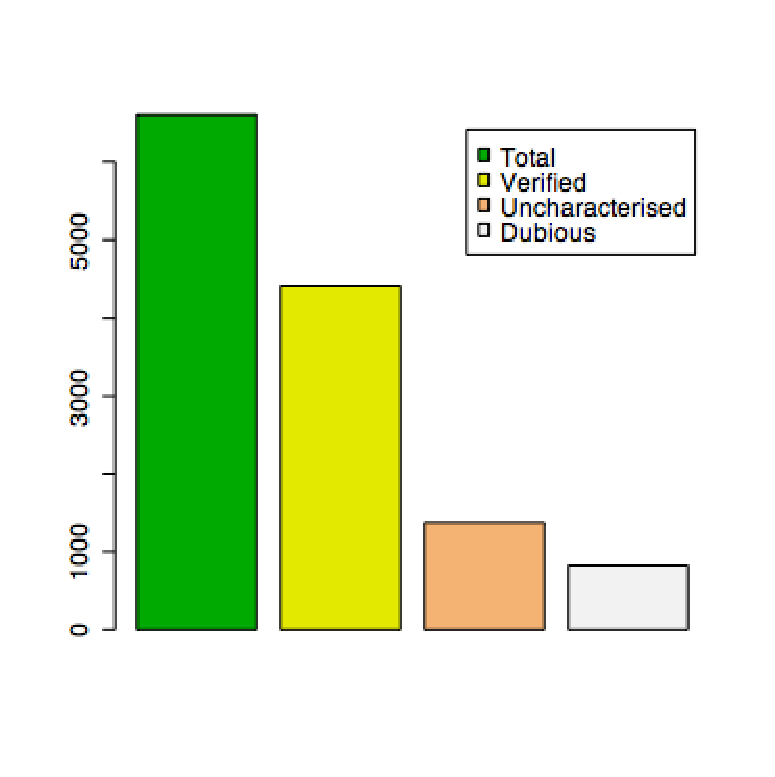
\includegraphics[scale=0.6]{sgd_orfs.eps}
\caption[ORF descriptions in the \emph{Saccharomyces} Genome Database]{Summary of ORF descriptions in the \emph{Saccharomyces} Genome Database, June 2006}
\label{figure:orf_totals}
\end{figure}

In \emph{S. cerevisiae}, as with other organisms, the field of functional genomics focuses on the identification and annotation of ORFs, the end goal being a complete map of all genes in the genome together with their role in cellular processes. Approaches to identifying genes often involve deleting the region of sequence thought to contain a gene, followed by identification of how the phenotype is affected; this method is aided by the simplicity with which specific sections of the yeast genome can be replaced via homologous recombination.

This technique, PCR-mediated targetted mutagenesis, relies on specific knowledge of the target region and the creation and insertion of a replacement cassette via PCR with a high degree of identity. This has the advantage that specific regions of sequence can be eliminated systematically, as well as the ability to completely remove the target gene which may not be the case using random insertional mutagenesis, described later. Furthermore, the incorporation of unique up and down tags for each mutant strain, as part of the insertion cassette, allows the amount of biomass of each mutant to be estimated by hybridisation of the extracted and PCR amplified tags using 5' prime radiolabelled nucleotides, this is outlined by Giaever \emph{et al.}\cite{giaever1999} and in figure \vref{insertion_outline} of this report \cite{delneri2004,wach1996,wach1994}.

The benefits of using the ``molecular barcode'' strategy is that quantitative measurements can be produced for each gene deletion mutant, where even small changes in growth rate compared to wild type can be identified, as opposed to qualitative fitness descriptions which are statistically less useful \cite{oliver2002,winzeler1999}. This strategy was used by an international consortium in 2002 to characterise phenotype under six conditions for homozygous deletion mutants for 96\% the \emph{S. cerevisiae} annotated ORFs \cite{giaever2002}. A paradigm for high-throughput functional genomics approaches this study determined which genes were essential to viability, as well as those that were non-essential but whose deletion resulted in a significantly slower growth rate.

Such large-scale studies, while providing large quantities of salient data, should not be considered a panopticon of gene and genome characterisation. Two \emph{in silico} studies of dispensability using genes involved in metabolism have shown that the essentiality of a gene depends both in what context the phenotype of the knockout is assessed as well as which other genes are present in the genome \cite{pal2006,papp2004}. Furthermore a study of ``silent'' mutations (genes whose deletion causes no discernible phenotype), showed that these deletions do have an effect on the concentrations of intracellular metabolites and that the role of the gene may be inferred from the levels of these metabolites within the cell \cite{raamsdonk2001}. These instances have led to further studies where homozygous gene deletant strains were grown in several different media and gene functional assignments were made over a range of contexts; the goal being to make inferences of under which conditions a gene is essential \cite{dudley2005,giaever2002}.

Another method of value in functional genomics is insertional mutagenesis based on randomly mutating stretches of the \emph{S. cerevisiae} genome in an \emph{Escherichia coil} plasmid, followed by excision and insertion into the the genome via mitotic recombination \cite{vidan2001}. This technique has the advantage that no prior knowledge of the target gene locations is required, and was usefully applied by Ross-Macdonald \emph{et al.} \cite{ross-macdonald1999} in identifying functional ORFs less than 50aa which had previously ignored due to the small size.

\subsubsection{Identifying gene function by partial suppression}

% Find out how many...
For certain genes under certain conditions deletion from the \emph{S. cerevisiae} genome results in an inviable mutant and therefore analysis of the homozygous deletant is not possible. This requires other strategies that allow the study of the role of the gene in cellular function; two techniques using the temporary or partial loss of gene function are the tetO-system and the construction of a hemizygous deletion mutant.

The tetO-system relies on the insertion of the \emph{tet} promoter upstream of the gene of interest. The activity of the genes under the control of the \emph{tet} promoter can be quantitatively controlled by the amount of doxycycline in the medium. The greater the quantities of doxycycline in the medium, the more the expression of the controlled gene is reduced. This allows the activity on the controlled genes to be precisely regulated by the concentration of doxycycline, and therefore the activity of the gene can be reduced without being completely removed \cite{mnaimneh2004}.

The second strategy, the construction of a heterozygous deletion mutant, where only a single allele in a diploid strain is replaced with the null cassette, allows the analysis of the role of even essential genes, again based on reduced activity. Using the same method as for homozygous deletion mutants, it is possible to measure the heterozygous phenotypic effects quantitatively, using continuous culture and quantitative measurement of the molecular barcodes. Similarly to the homozygous mutant genome survey, heterozygous mutants were created for $\sim$5900 yeast ORFs and compared to wild-type growth in batch culture. Approximately 3\% of genes showed a reduced growth rate, half of these being annotated as being involved in metabolic processes \cite{deutschbauer2005}. This figure however has been proposed to to be much higher 10\% - 12\%, when using a growth rate controlled continuous culture instead \cite{papp2006}.

\subsection{Understanding gene function \emph{in silico}}

Determining the function of gene \emph{in silico} has the advantage over experimental approaches of being relatively faster and cheaper. Infering gene function through sequence similarity using BLAST \cite{blast} is widespread in molecular biology and the field of bioinformatics has developed genome wide comparisons \cite{blat} or more sensitive hidden markov model based searches \cite{hmmer}.

A systems biology approach to functional genomics will focus on the context of a gene in a dynamical system. In comparison to the described approaches for identification of essentiality \emph{in vivo}, a similar approach can be applied \emph{in silico} using flux balance analysis of genome scale metabolic models. Removal of a reaction in a genome scale model can be used to simulation the \emph{in vivo} process of gene knockout, as no flux can proceed through the reaction. When performed in the yeast genome scale model XXX \% of knockout phenotypes were correctly predicted. The advantage of using \emph{in silico} models is that even large scale functional genomic approaches can be performed easily. 

Genomic redundancy, where more than gene provides the same function, can be tested \emph{in vivo} through combined double deletion of gene pairs. In theory this would require ~6600$^2$ deleteion and be work intensive. Performin this \emph{in silico} is that this process would require only a little more time than the performing single deletions \emph{in silico}. Harrison \emph{et al.} \cite{double_deletion} showed that this approach can predict XXX \% of \emph{in vivo} double deletion phenotypes.

Genome scale models are well suited to the prediction of knockout phenotypes as there is a direct correspondence between the removal of a gene from the genome and the removal of the encoded enzyme in the metabolic network. When predicting phenotypes which are not simply a case of either on or off for the gene the analysis will be more complex. As an example gene dosage dependency can be analysed \emph{in vivo} through removal of one of the allelic copies of the gene. Performing this analysis with a genome scale model will be more complicated as the removal of half a gene does not translate so easily to the metabolic network. As example the removal of half a gene can be hypothesised not to result in a 50\% reduction in enzyme activity as transcription and translation of the gene may not follow linear dynamics, and even if this were the case enzyme kinetics often follow a non-linear response curve.

In addition to the above example of predicting haploid phenotypes, studying and predicting evolutionary effects in terms of the metablic network is also of interest. A substitution in the sequence of an enzyme encoding gene may have an effect on the corresponding kinetics of the encoded enzyme if the subsitution is in a region effecting the enzymes structure. The more important to growth, the greater the effect the mutation will have the competition of the organism in the environment. Therefore it may be possible to predict the selection pressure on the encoding gene based on the relevence to the phenotype of the organism. Similarly a mutational effect may not necessarily change the encoded protein sequence, but instead affect the rate at which the enzyme is translated through modification of the adaptation of the transcript for translation.

In Chapter 2 an approach was described using genome scale metabolic to estimate the control gene encoded reaction on the nutrient uptake fluxes of the organism. Using a subset of the reactions in the model that are encoded by a single gene, the relationship between the gene and the reaction is one to one. This should mean that any changes in the gene sequence should be directly reflected in the metabolic phenotype, this may not necessarily be the case if there were a homologue catalysing the same reaction. Therefore these gene cost measures can be tested to see if they reflect any the selection pressures described above. This may provide an indication if genome scale models and flux balance analysis are suitable techniques for making inferences about the evolution of gene sequence.

\subsection{Summary of results}

In this chapter the estimated gene costs from Chapter 2 are compared with a number of biological characteristics. First estimated gene cost is compared with data estimating the dosage dependency of yeast genes. Next the gene cost is compared with the estimated expression level of the gene. Finally gene cost is compared with evolutionary rate of the gene.

\section{Results}

\subsection{Gene sensitivity and haploinsufficiency}

\subsection{Gene sensitivity and expression}

\subsection{Gene sensitivity and evolutionary rate}

\section{Discussion}

\section{Materials and Methods}
